\chapter{Background}\label{background}
This chapter provides an overview of the concept of sharing systems and how they have evolved into an important part of urban life. \Cref{micromob} provides a general description of the concept of micromobility, followed by an overview of different sharing systems and their historical progress in \Cref{sharing}. Further, \Cref{escooters} describes the history of e-scooters as a micromobility service and concepts related to their use. Finally, \Cref{challenges} discusses challenges related to e-scooter sharing systems. 

\section{Micromobility}\label{micromob}

Global urbanization is rising and over half the world’s population now lives in cities \citep{zarif_small_2019}. Thus, the need for additional methods of transportation has been apparent the past decades. Simultaneous as a growing environmental focus, the use of micromobility services has risen. Micromobility vehicles are typically used as a supplement to traditional public transportation, offering first- and last-mile transportation opportunities. As traffic congestion in cities is on the rise, the traditional public transportation in many places can no longer keep up with the growing population. Thus, many people look for opportunities in micromobility services, both as a substitute for public transportation and as a way of connecting with the network of transportation options already available.

\subsection{What is Micromobility?}
Micromobility refers to a wide range of different small and lightweight vehicles. They operate at a relatively low speed, typically below 25 km/h. The term micromobility has historically been used to describe bicycles, e-scooters, electric skateboards, and more. However, in most markets today, micromobility relates to shared bicycles and e-scooters. Micromobility vehicles have been around for centuries, from the invention of the first bicycle to the wide variety of electric vehicles people use for transportation today. Still, it is only in the last couple of years that these vehicles have emerged as a serious alternative for urban mobility. The growth is mainly driven by the advances in battery and GPS tracking technology, along with the widespread use of smartphones. 

E-scooters in particular, have had their popularity increase over the past years, with multiple operators emerging in most major cities. Their rapid growth is almost unprecedented in the transportation sector, with Bird, as one of the first operators, hitting 10 million rides within their first year of operating in Southern California. 

\subsection{The Environmental Impact of Micromobility}\label{impact}
Traffic congestion results in a significant amount of lost time across the globe. In 2014 heavy traffic caused an extra 6.9 billion travel hours for Americans in the US alone, and consequently caused an additional consumption of 11.7 billion liters of fuel. This problem has grown significantly worse in the past decades \citep{bopp_bicycling_2018}. Micromobility services contributes to solving this problem, in the form of smaller and simpler means of transportation. They allow for a higher number of transportation vehicles in the cities, while at the same time reducing the space occupied. 

 If the alternative transportation for a user is to use a car, micromobility vehicles offer a greener alternative.  The energy efficiency is the main reason for this.  According to a 2016 study  by  the  US  Department  of  Energy,  the  average  American  car  weighs  around  23  times  as much  as  the  person  it  moves \citep{tillemann_forget_2018}.   Comparing  this  to  an  average of 12  kg  e-scooter, the e-scooter  provides  a  much  more  energy  efficient  way of transportation.  In fact, e-scooters offer such a high level of energy efficiency, that the average human would burn around 9 times as much energy walking a given distance, as an e-scooter would driving it. \Cref{fig:magnitude of efficiency} illustrates the efficiency of e-scooters compared with other means of transportation.
\\
\begin{figure}[H]
    \centering
    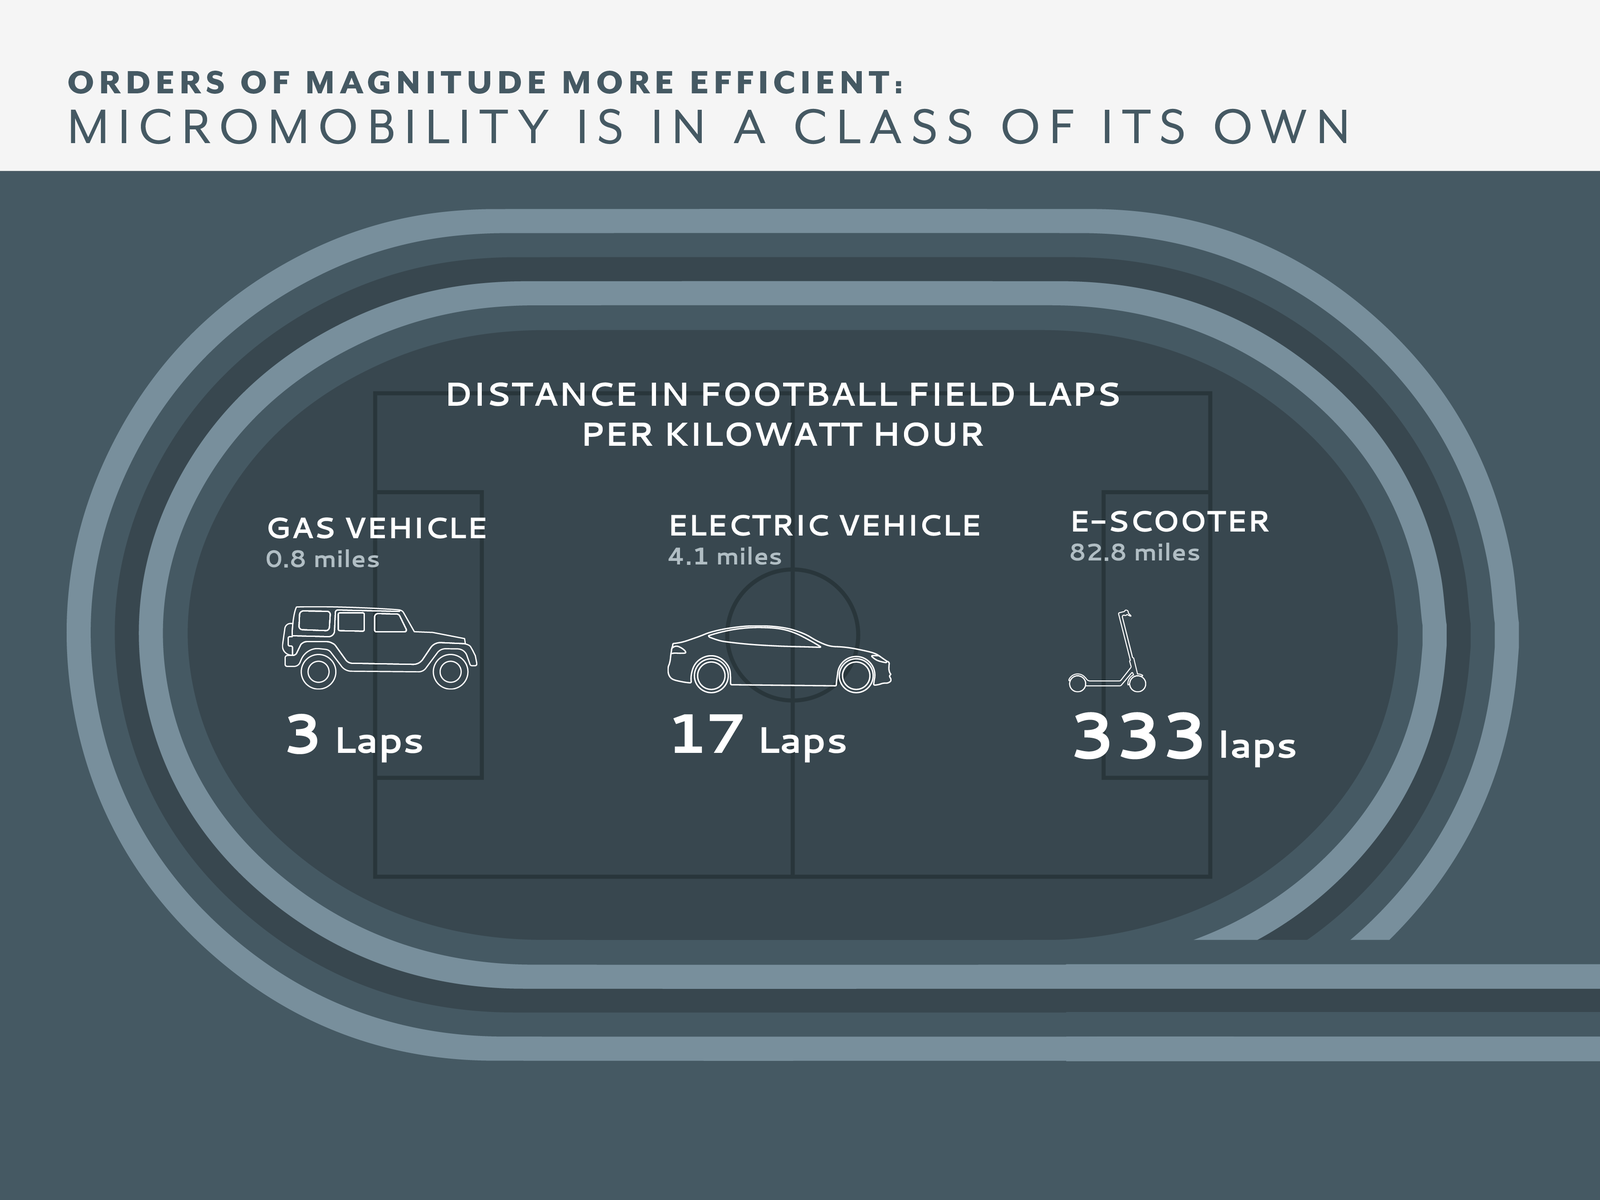
\includegraphics[width=0.8\columnwidth]{Images/footballfields.png}
    \captionsource{ Illustration of the energy efficiency of different methods of  transportation.}{\citet{tillemann_forget_2018}}
    \label{fig:magnitude of efficiency}
\end{figure}

The cost of fueling and production underlines the environmental benefit of electric micromobility vehicles. Roughly 60 percent of trips in the US are shorter than 8 km, which speaks to the advantage of micromobility, as traveling relatively short distances is the main use of lighter vehicles. In addition, each micromobility vehicle is cheaper and less costly to produce and accounts for less CO2 emissions than its heavier counterpart, thus adding to the positive impacts related to short-distance traveling (\Cref{fig:cars_scooters}). These benefits are definitely some of the reasons why the popularity of these vehicles is rapidly growing, and are projected to grow also in the future. 
\\
\begin{figure}[H]
    \centering
    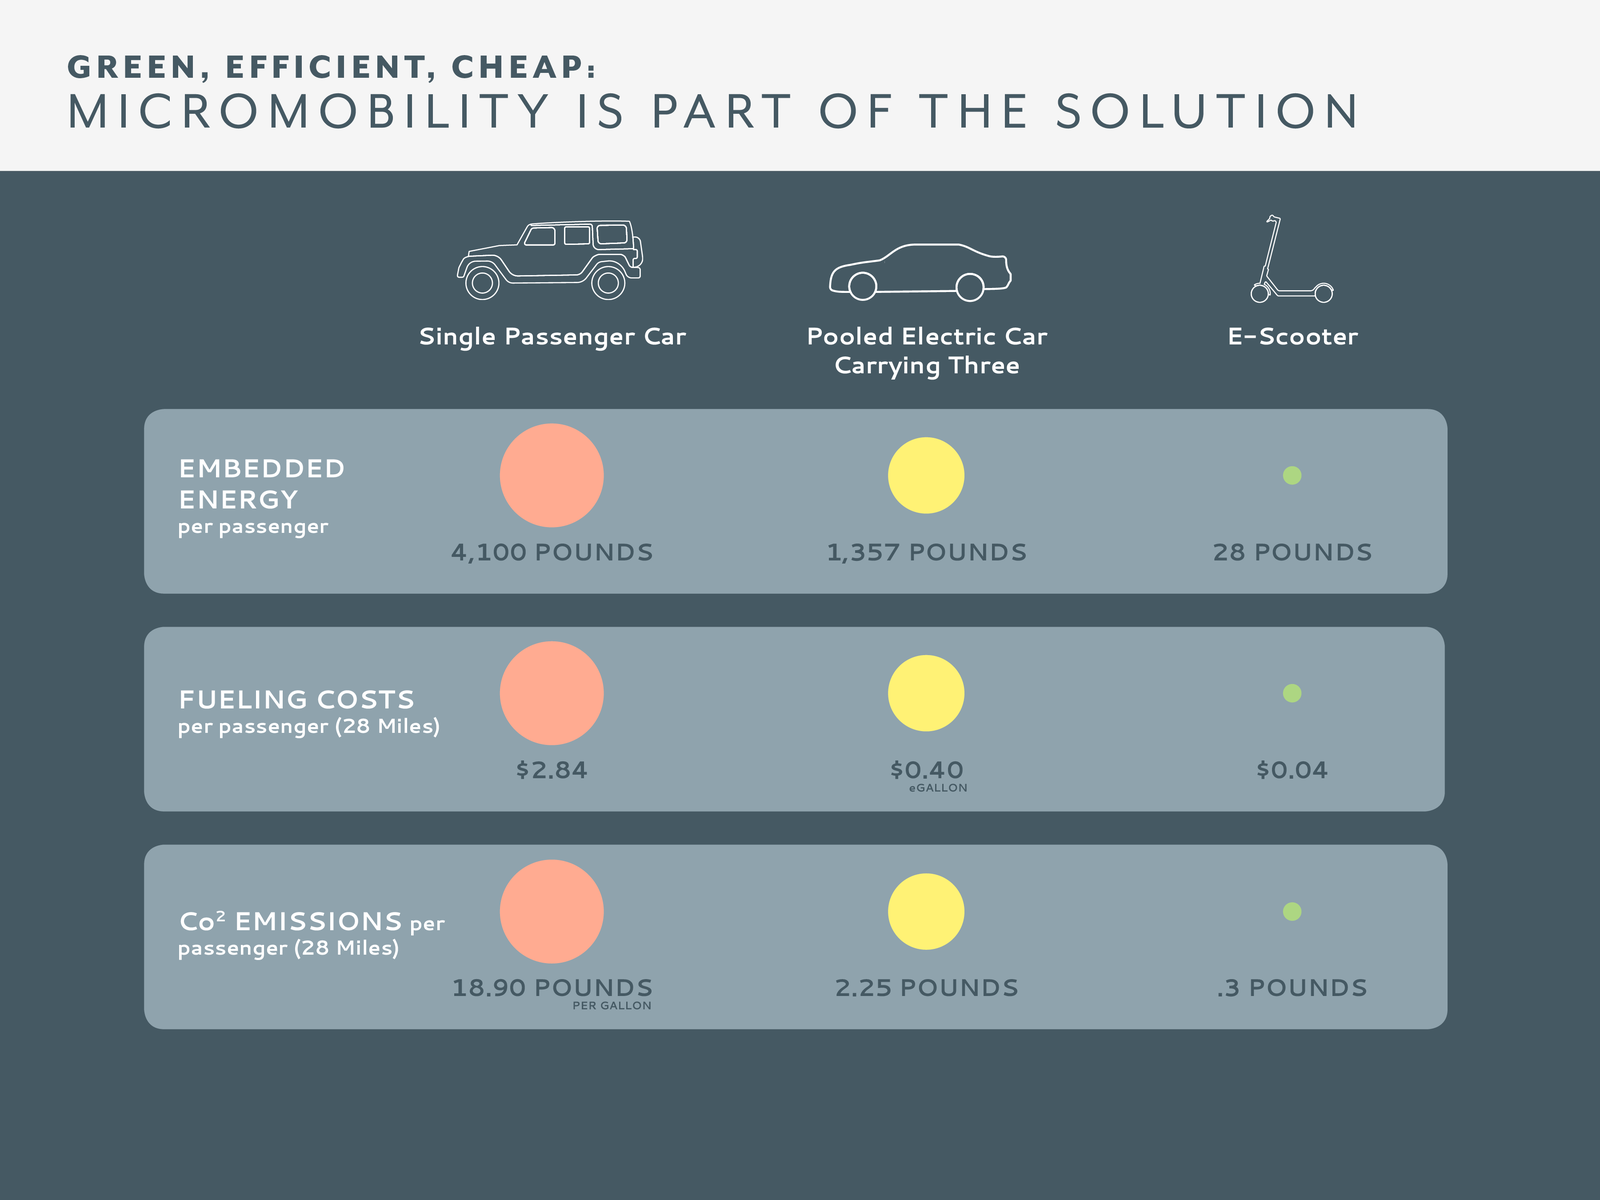
\includegraphics[width=0.8\columnwidth]{Images/carsscooters.png}
    \captionsource{The environmental impact of different methods of  transportation.}{\citet{tillemann_forget_2018}}
    \label{fig:cars_scooters}
\end{figure}

Although the cost of production and fueling is low, the environmental impact of doing so is negative.  \citet{hollingsworth_are_2019} discuss the impact of micromobility on the environment in detail, focusing on e-scooters. They conclude that, despite the positive environmental effects of riding an e-scooter, the manufacturing and operation of charging, maintaining, and rebalancing the e-scooters' dominate their environmental impact.

However, through some improvements, the environmental burden can be eased significantly. Naturally, Hollingsworth and his coauthor's model is highly sensitive to e-scooter lifetime \citep{hollingsworth_are_2019}. Newer, sturdier and longer-lasting e-scooters will thus have a positive impact on the environment, locally and globally, as well as being the economically viable option. Nevertheless, the issue that yields the most significant negative impact is the collection and charging approaches used by the operators. Hollingsworth and his coauthors suggest that improvements to these approaches would drastically improve the environmental footprint of e-scooter systems. The introduction of swappable batteries, as opposed to charging an e-scooter at the depot, has been a move in the right direction. However, Hollingsworth and his coauthors stress the importance of the battery swapping and relocation operation. These operations are today often done on a local level, without a plan, and thus, are seldom optimal.

\section{Sharing Systems}\label{sharing}

Sharing systems can include services of different kinds, but this report focuses on sharing systems related to micromobility. These are mainly dominated by Bike Sharing Systems (BSS)  and E-scooter Sharing Systems (ESS). Historically, BSS have been more common than ESS, but in the past couple of years, ESS have emerged in great numbers.

The sharing systems of today provide short-term rental of micromobility vehicles within a defined geographic area. BSS are typically constrained by a set of stations where the bicycles are available for pick-up and drop-off. Although these station-based systems have dominated the BSS market, certain Free-Floating Sharing Systems (FFSS) are also present. The FFSS typically consists of electrical micromobility vehicles containing GPS services to keep track of their position. ESS is a free-floating system. Hence, the e-scooters are spread out across a city based on expected demand in different areas. Today, they are typically placed in certain hot-spots determined by historical demand and the experience of the operators. This is opposed to BSS where the placement of the bicycles is constrained to their stations. 

Customers wanting to use a bicycle or an e-scooter does so through an application on their smartphone, connected to the BSS or ESS. After downloading the application and registering their account, they will see a real-time mapped view of available vehicles. Further, unlocking the vehicle before riding is done through the application, as well as locking it after use. When the customer has reached their destination, they can place the e-scooter where they want, as long as they are parked inside the company's geographical boundary. The application provides the operators with valuable data on the use patterns and status of the vehicle fleet. \Cref{fig:application} visualizes the process of renting an e-scooter in the described application. The first two steps are only performed once, while the remaining steps are repeated for each rental. 
 \\
\begin{figure}[H]
    \centering
    
\includegraphics[width=0.9\columnwidth]{Images/user_interaction.png}
    \caption{The user-interaction process to unlock and ride an e-scooter.}
    \label{fig:application}
\end{figure}

As discussed in \Cref{impact}, the environmental footprint of transportation vehicles is becoming increasingly important with a growing urban population. Sharing systems designed around micromobility vehicles have a positive impact on this issue. First of all, sharing systems decrease the total amount of transportation vehicles needed to satisfy the total demand for transportation in a city. Sharing systems do this by lowering the amount of time transportation vehicles are left unused, and maximizing the usability of the vehicles. Fewer vehicles lead to less traffic congestion, less local pollution, and less space being occupied in a city. As a consequence, sharing systems are an economically efficient and low-cost way of satisfying demand. 

A free-floating system accounts for fewer barriers to entry. Not having to invest in building stations leads to smaller initial costs and fewer regulations and legislations to surpass before entering the market. Additionally, the scalability of the market is high. Low amounts of funds are needed for each extra e-scooter added to an operator's fleet. These factors lead to a market characterized by a large number of participants with a big fleet of vehicles, as is seen in many cities worldwide. 


\section{E-Scooters}\label{escooters}

The history of e-scooters dates back to 1895 when Ogden Bolten Jr patented the first electrical driven scooter, but it would take over 100 years before the e-scooter we use today was introduced. In early 2000, Go-Ped launched the first e-scooter and 15 years later the refined e-scooter became common property. The evolution of the e-scooters is driven by lighter and stronger construction and better battery technology. Today, e-scooters can travel up to 80 km/h and have a range of over 100km depending on weight and area of use. The more common commercial variants have a range of around 40-60 km and a speed limit of 25 km/h. 

E-scooters available for rent were first introduced in a sharing system in Santa Monica Hall US in September 2017 \citep{hall_bird_2017}, and later to the global market. These e-scooters became successful by making short distance travel faster and more energy efficient. The main business idea of the e-scooter companies is to distribute e-scooters in popular and crowded areas for customers to use. 

The use patterns of e-scooters are different in the US compared to the European market. \citet{caspi_spatial_2020}, examining Austin, Texas, suggest that the usage of e-scooters is not associated with commuting, but rather for recreational use, tourism, and a substitute for walking. \citet{mathew_analysis_nodate}, \citet{mckenzie_spatiotemporal_2019}, and  \citet{noland_trip_2019} support this claim in other major cities in the US. TØI argue that this is slightly different in Norway due to the extensive use of public transport, availability of parking spots, and general environmental focus \citep{fearnley_delte_2020}. 

During the last year, e-scooter companies have made an important change to their fleet. Now, replaceable batteries are entering the market \citep{tier_mobility_tier_2019}. The e-scooter companies can operate by only replacing batteries on the e-scooter's location without collecting the e-scooter for charging overnight at a warehouse. This new model changes how these companies operate. Needed space for charging at the depot is drastically reduced, making it easier for the companies to scale up. 

Maintaining the fleet of e-scooters has always been a concern for the e-scooter companies. In the early models that were introduced in 2018, all e-scooters had to be picked up by the company and recharged at a depot. In the US, companies paid private persons to pick e-scooters up at night, charge them at home and place them out in dedicated “hubs”. This model has not been adopted in Norway, where charging of e-scooters is done by the operators themselves (see \Cref{e-scooters in norway}). The operators use a fleet of vehicles that either carry only batteries or both batteries and e-scooters around in the city. We refer to these vehicles as service vehicles henceforth. 

\subsection{E-scooters in Norway}\label{e-scooters in norway}
As our project is focused on the Norwegian e-scooter industry, we want to take a closer look at the market dynamics in Norway and more specifically, Oslo. Through conversations with two major operators in Norway it has become clear that the main focus of operation is availability of e-scooters. Operators are loosing income if they cannot supply e-scooters for their users at any time. In a growing industry with almost homogeneous products and services, the operators strive to always meet user demand.

The e-scooter operators in Norway utilize different business models. The most common way to charge customers for riding an e-scooter is with a fixed price for unlocking the e-scooter and an additional  price for each minute used. Operators have also introduced monthly passes, which include unlimited free rides in exchange for a monthly fee. Loyalty programs that give customers a discount on the fixed or variable price in stepwise tiers is also utilized to encourage use. Additionally, to attract new customers, referral programs that reward existing customers with credits when they enroll friends have been adopted by the industry players.

Oslo was the first city where e-scooters were introduced in Norway. Early in the spring of 2019 TIER and Voi entered the Norwegian market. Since then, nine additional operators have joined the competition, expanding to the cities of Bergen, Trondheim, Stavanger, and Drammen. The Norwegian government has not approved any national law to regulate the e-scooter industry, and have decided on a “wait and observe”-strategy before any legislation is going to be approved. The local government in both Trondheim and Bergen has tried to regulate use and licenses inside the city's boundaries without any luck (see \Cref{challenges}).  

Most operators place their e-scooters in the city center during the night to rebalance their fleet. According to \citet{fearnley_delte_2020} 86 percent of deployment of e-scooters happens during the night, and e-scooters are mainly deployed close to the city center and public transport stations. This is backed by looking at where most trips are started in the morning. Places like Bogstadveien, Bislett, Aleksander Kiellands Plass, Nationaltheateret, Aker Brygge, and Oslo S stands out. The operators clearly focus on the central areas and not on residential areas.

E-scooters in Oslo are mainly used to solve the last mile problem \citep{fearnley_delte_2020}. The last mile problem is defined as completing the final part of a trip. E.g people that use public transport to work often make use of e-scooters to take them from the station to their workplace.  \citet{fearnley_delte_2020} shows that there is extended use of e-scooters from Oslo central station to Barcode where large corporations like DNB, Microsoft, and PwC have their offices. They have also discovered that the average end-time of a trip is skewed to the end of the hour with a little increase in the half-hour. This reveals that e-scooters in Oslo often are used as a last-minute transport to meetings and appointments. 

In Oslo, e-scooters are mainly used as a substitute for public transportation, walking and taxi rather than for recreational use. \citet{fearnley_delte_2020} conclude that the usage of e-scooters in Oslo is higher on weekdays than on weekends supporting the claim of non-recreational use. \Cref{fig:TOI_trips} shows the general use of e-scooters in Oslo. Usage increases almost continuously to around 5 pm, with a small peak around 9 pm, and slowly decreases to 11 pm when the e-scooters are locked and not able for use in Oslo. This demonstrates the importance of having an e-scooter fleet that has enough battery percentage to meet the demand throughout the whole day. 
 \\
\begin{figure}[H]
    \centering
    \includegraphics[width=0.9\textwidth]{Images/TØI_trips_Oslo.png}
    \captionsource{Average Number of trips in Oslo during the day.}{\citet{fearnley_delte_2020}}
    \label{fig:TOI_trips}
\end{figure}


\subsection{Charging Stations}\label{sharging stations}

The newest addition to the e-scooter industry is the introduction of charging stations for customers to charge the e-scooters. TIER has started a pilot project in Tampere, Finland, where they cooperate with shops and cafes. The shops are hosting small charging stations so customers can swap discharged batteries with fully charged batteries \citep{plikk_slik_2019}. Another way to implement this self-charging strategy is with charging racks, where customers can place their e-scooters after the end of a trip. These racks can be powered by hooking them up to the local grid or solar panels. 

By introducing charging stations, users can change the batteries themselves. This will, hopefully, create an organic system where the operator does not need to swap batteries, resulting in a cost reduction. For this to work, some kind of incentive for the customers to change the batteries would have to be in place, as well as a method to prohibit theft of batteries. The incentives can vary, but the most logical way is with free or discounted trips. 

One of the challenges e-scooter companies may face implementing charging racks is public regulations. If every e-scooter brand introduce their own charging stations in cities, the cities could be filled with these stations polluting the streets. Setting up racks in public areas requires approval from the local government and this can be a time-consuming process. We may have to wait years to see this coming, but with more and more cities introducing licenses to operate, this could help speed up the process. Charging stations can be a game changer for the e-scooter industry and an area of research with interesting opportunities.  

The willingness of customers to charge e-scooters could vary from city to city. As the consumers in Oslo often use e-scooters as a last-minute method of transportation, it is unlikely that the willingness to spend additional time charging batteries themselves is going to be very high. This reduces the probability of success of launching portable chargers in Oslo. Thus, this report will not conduct further research on this topic.

\section{Challenges with E-scooters}\label{challenges}

By 2020, electrical scooters are available in all major cities in Europe and the US. Being an attractive market for investors and venture funds, the competition for the e-scooter customers has been substantial since the introduction in 2017. Consequently,  vast amounts of e-scooters has been dumped up in the streets of various American and European cities to gain market share. E-scooters blocking sidewalks, overfilling parks, and deserting to become litter are some of the problems cities have encountered during this boom. These problems have raised a large number of complaints against rentable e-scooters causing a demand for regulatory provisions. 

Cities and local governments have dealt with the problem of littering and overflow of e-scooters in different ways, with various outcomes. In Trondheim, Norway, the local government made it illegal to rent out e-scooters without a license \citep{shifter_trondheim_2020}. However, e-scooter operators have ignored these licenses and have kept on operating in Trondheim. Due to not having any leagal basis, the local government in Trondheim has no way of stopping them keeping all operators still in service. In Bergen, the local government lost in court to the operator Ryde trying to refuse them to operate in the city without a license \citep{ntb_bergen_2020}.  Until a national law regulating the e-scooter market is passed, the e-scooter market is free for all in Norway. In October 2020, the local government of the Danish capital, Copenhagen, banned the e-scooters at public property in central Copenhagen. Operators in Copenhagen are restricted to rent out e-scooters from designated spots in the city center and have to ensure the users place them back at these spots after usage.

Micromobility is a young and growing industry where regulations will shape its future. As we have already seen, tender processes will most likely be a part of the market dynamics, pushing the margin for e-scooter companies down. Since the dawn of the e-scooter industry, companies have struggled to be profitable. One of the largest American operators, Lime, reported a loss of \$300m with a corresponding \$420m in revenues \citep{wilhelm_as_2019}. The Swedish company Voi reported a positive operational profit in June 2020, but the 2019 report showed that they lost nearly SEK 770m \citep{johannessen_voi_2020}. These numbers emphasize the tough competition and that the market is up for great changes. For regulatory and economic reasons, we observe the importance of optimized and cost efficiency for the industry going forward. 
